% Zadnja posodobitev: 14. 1. 2022
\documentclass[twoside,11pt]{article}
\usepackage[slovene]{babel}
\usepackage[utf8]{inputenc}
\usepackage{graphicx}
\usepackage[frame]{matrika}
\usepackage{mathtools}
\usepackage{epstopdf}
\usepackage{units}
% Po potrebi se lahk dodajo drugi standardni paketi, ki ne spreminjajo izgleda dokumenta

\usepackage{bbm}
\usepackage{tikz}
\usetikzlibrary{positioning, 
                arrows.meta,                % arrow tips
                intersections,              % find intersection between paths
                spath3} % split and transform paths



\begin{document}

\MAT{1}{11}{2024}
\naslov{Brownovo gibanje}

\avtor{Anej Rozman}

\institucija{Fakulteta za matematiko in fiziko \\ Univerza v Ljubljani}

\klasifikacija{~} 
\izvlecek{
    V članku motiviramo idejo Brownovega gibanja in podamo njegovo matematično definicijo. 
    Predstavimo in doka"zemo nekaj osnovnih lastnosti ter rezultatov, kot je simetričnost Brownovega gibanja, "cas ustavljanja, krepka lastnost Markova,
     princip zracljenja in presenetljiv rezultat, da je realizacija Brownovega gibanja nedovedljiva funkcija.
     }  
\title{Brownian motion}
\abstract{
    In this paper we motivate the idea of Brownian motion and give its mathematical definition. 
    We present and prove some basic properties and results, such as the symmetry of Brownian motion, stopping time, strong Markov property,
    reflection principle and the surprising result that the sample path of Brownian motion is an undifferentiable function.
    }

\glava\baselineskip=14.5pt

\smallskip

\section{Uvod}

Določeni posebni primeri slučajnih procesov so skozi zgodovino doživeli obsežen
matematični razvoj. Brownovo gibanje je najbolj znano in zgodovinsko prvo, ki je bilo 
temeljito raziskano. Kot fizičen pojav je
bilo Brownovo gibanje odkrito s strani angleškega botanika Roberta Browna leta 1827.
Matematični opis tega pojava je bil prvič izpeljan iz fizikalnih zakonov s strani 
Einsteina leta 1905. Od takrat je področje doseglo znaten napredek. Fizikalno teorijo 
so nadalje izpopolnili Fokker, Planck, Ornstein in drugi. Matematična 
teorija je počasneje napredovala, ker je natančen matematični opis modela postavljal 
težave, medtem ko so bila nekatera vprašanja, na katera so fiziki iskali odgovore na
podlagi tega modela, precej preprosta in intuitivna. Na veliko vpra"sanj je odgovoril Bachelier
v njegovi disertaciji leta 1900.
Prvo jasno matematično formulacijo teorije pa je Wiener podal v svoji
disertaciji leta 1918 in kasnejših člankih, zato je alternativno poimenovnanje 
Brownovega gibanja Wienerjev proces. Je primer slučajnega procesa, ki se danes skupaj z 
njegovimi posplošitvami pojavlja na številnih področjih kot so biologija, finance, fizika,
itd. V članku se bomo osredotočili na matematično izpeljavo osnovnega Brownovega gibanja 
na $\mathbb{R}$ ter nekaj lastnosti in ne na uporabo v že prej omenjenih področjih.
Prvo pa si poglejmo nekaj osnovnih defnicij, ki jih bomo potrebovali v nadaljevanju.

\begin{definicija}
    Naj bo $(\Omega, \mathcal{F}, \mathbb{P})$ verjetnostni prostor in naj bo $T\neq\emptyset$ neprazna
    indeksna množica ter $(S, \Sigma)$ merljiv prostor. \textit{Slučajni proces}, parametriziran
    s $T$, je družina slučajnih spremenljivk $X_t : \Omega \to S$, ki so $(\mathcal{F}, \Sigma)$-merljive
    za vsak $t \in T$.
\end{definicija}

\begin{opomba}
    Za naše namene bomo privzeli, da je $T = [0, \infty), \ (\mathcal{F}, \Sigma) = (\mathbb{R}, \mathcal{B}_{\mathbb{R}})$,
    kjer $\mathcal{B}_{\mathbb{R}}$ predstavlja Borelovo $\sigma$-algebro na $\mathbb{R}$. 
\end{opomba}
    
\begin{definicija}
    Za fiksen $\omega \in \Omega$ je preslikava 
    $[0, \infty) \rightarrow \mathbb{R}; \ t \mapsto X_t(\omega)$ 
    \textit{realizacija} slučajnega procesa $(X_t)_{t\geq0}$.
\end{definicija}

%\begin{opomba}
%    Na slu"cajni proces lahko gledamo tudi kot na predpis, ki nam iz vor"cnega prostora 
%    $\Omega$ priredi slu"cajno funkcijo $(X_t(\omega))_{t\geq0}: [0, \infty) \rightarrow \mathbb{R}$.
%\end{opomba}

\pagebreak

\section{Motivacija in definicija Brownovega gibanja}

Kot Robert Brown si za motivacijo oglejmo naključno gibanje delca v $\mathbb{R}^2$.
Zaradi preprostosti bomo zahtevali, da se gibanje začne v koordinatnem izhodišču. Želeli bi tudi, da so 
poti delca zvezne, saj nam nenadni skoki nebi pomagali pri opisovanju pojava.  

\begin{figure}[h]
    \centering
    \begin{tikzpicture}
      \draw[->] (-1,0) -- (6,0) node[right] {$x$};
      \draw[->] (0,-1) -- (0,4) node[above] {$y$};
  
      \draw[thick,blue] plot[smooth,tension=0.8] coordinates {(0,0) (1,2) (2,1) (3.3, 2.6) (3,3) (2.5,2) (5,2) (6,3.2)};

      \filldraw[black] (6,3.2) circle (1pt);

      \node[above ,black] at (6,3.2) {$\left(B^x_{t}, B^y_{t}\right)$};
    \end{tikzpicture}

    \caption{Gibanje delca v xy-ravnini.}
    \label{fig:slika1}
\end{figure}

\noindent
Označimo z $\left(B^x_{t}, B^y_{t}\right)$ položaj delca v času $t \geq 0$. Ker se delec v vse 
smeri giblje z enako verjetnostjo, bo pričakovana vrednost pozicije enaka $\mathbb{E}\left[(B_t^x, B_t^y)\right] = (0, 0).$
Smiselno bi bilo privzeti, da so premiki delca med seboj neodvisni, torej, 
da gibanje med časom $0$ in $t_1$ (razen tega kje gibanje začnemo) ne vpliva na gibanje med časom $t_1$ in $t_2$ in tako naprej.

\begin{definicija}
    Naj bo $(X_t)_{t\geq0}$ slu"cajni proces. Potem za $s < t$ definiramo \textit{prirastek procesa} $X_t - X_s$ na 
    intervalu $[s, t]$. Proces $(X_t)_{t\geq0}$ ima \textit{neodvisne prirastke}, če so za vsak nabor 
    $0 \leq t_1 < t_2 < \ldots < t_n < \infty$ prirastki (slučajne spremenljivke)
    $$
        X_{t_2} - X_{t_1}, \ X_{t_3} - X_{t_2}, \ \ldots, \ X_{t_n} - X_{t_{n-1}}
    $$
    med seboj neodvisni.
\end{definicija}

\noindent
V na"sem primeru to zapišemo, da so vektorji $(B^x_{t_2}, B^y_{t_2}) - (B^x_{t_1}, B^y_{t_1}), \ \dots, (B^x_{t_n}, B^y_{t_n}) - (B^x_{t_{n-1}}, B^y_{t_{n-1}})$
med seboj neodvisni. Prav tako bi bilo smiselno privzeti, da "ce si izberemo nek "casovni interval $[s, t]$,
 je porazdelitev prirastka odvisna le od dol"zine tega "casovnega intervala in ne od tega, kje gibanje gledamo. 

\begin{definicija}
    Naj bo $(X_t)_{t\geq0}$ slu"cajni proces. Potem pravimo, da ima proces \textit{stacionarne prirastke}, "ce za vsak $s < t$ in vsak $h > 0$ velja, da ima $X_{t+h} - X_{s+h}$ enako porazdelitev kot $X_t - X_s$.
\end{definicija}

\noindent
Če to velja vidimo, da je $\left(B^x_{t}, B^y_{t}\right)$ vsota neodvisnih prirastkov. Po centralnem 
limitnem izreku bi torej pričakovali, da je vektor $\left(B^x_{t}, B^y_{t}\right)$ normalno porazdeljen.
Spomnimo se, da je slučajna spremenljivka $X$ normalno porazdeljena s pričakovano vrednostjo $\mu$ in varianco $\sigma^2$, če
je njena gostota porazdelitve enaka
$$
    f_X(x) = \tfrac{1}{\sqrt{2\pi\sigma^2}}\exp\left[-\tfrac{(x-\mu)^2}{2\sigma^2}\right].
$$
Zaradi neodvisnosti prirastkov bo tudi $\text{Var}(B_t^x) = \text{Var}(B_t^y) = t$, torej odvisna le od tega koliko časa opazujemo delec.
Ta razmislek nas privede do definicije Brownovega gibanja na $\mathbb{R}$, kjer bi ga radi matematično karakterizirali.

\pagebreak

\begin{definicija}
    Slučajnemu procesu $(B_t)_{t\geq 0}$ definiranem na verjetnostnem prostoru $(\Omega, \mathcal{F}, \mathbb{P})$
    z vrednostmi v $\mathbb{R}$ pravimo \textit{Brownovo gibanje}, če 
    zadošča naslednjim pogojem:
    \begin{enumerate}
        \item $\mathbb{P}(B_0 = 0) = 1$,
        \item realizacije $(B_t)_{t\geq0}$ $(t \mapsto B_t)$ so $\mathbb{P}$-skoraj gotovo zvezne,
        \item proces $\left(B_t\right)_{t \geq 0}$ ima neodvisne prirastke t.j. za $0 \leq t_1 < t_2 < \ldots < t_n < \infty$ so slučajne spremenljivke
            $B_{t_2} - B_{t_1}, \ B_{t_3} - B_{t_2}, \ \ldots, \ B_{t_n} - B_{t_{n-1}}$ med seboj neodvisne. 
        \item Za $ 0 \leq s < t < \infty$ je $B_t - B_s \sim N(0, t-s)$.
    \end{enumerate}
\end{definicija}
        
Vprašanje, ki se nam porodi je, ali sploj obstajta verjetnostni prostor 
in slučajni proces, ki zadoščata zgornjim zahtevam. Odgovor je pritrdilen in ga 
podamo v obliki izreka.

\begin{izrek}
    Obstaja verjetnostni prostor $(\Omega, \mathcal{F}, \mathbb{P})$ in
    izbira slučajnih spremenljivk $B_t : \Omega \to \mathbb{R}$ za $t \geq 0$,
    ki ustrezajo definiciji Brownovega gibanja.
\end{izrek}

\begin{dokaz}
    Dokaz izreka je precej tehničen in nezanimiv za namen članka, zato ga bomo izpustili. Najte"zji del je 
    pokazati, da so realizacije zvezne. Lahko ga najdemo v \cite{1}. $\hfill \square$
\end{dokaz}


Od sedaj naprej bomo vedno z $(B_t)_{t\geq 0}$ ozna"cili Brownovo gibanje, ki bo vedno definirano na 
verjetnostnem prostoru $(\Omega, \mathcal{F}, \mathbb{P})$ in se nanj (razen po potrebi) ne 
bomo sklicevali. Priročno bo v mislih držati sliko realizacije  \ref{fig:slika2}.

\begin{figure}[h]
    \centering
    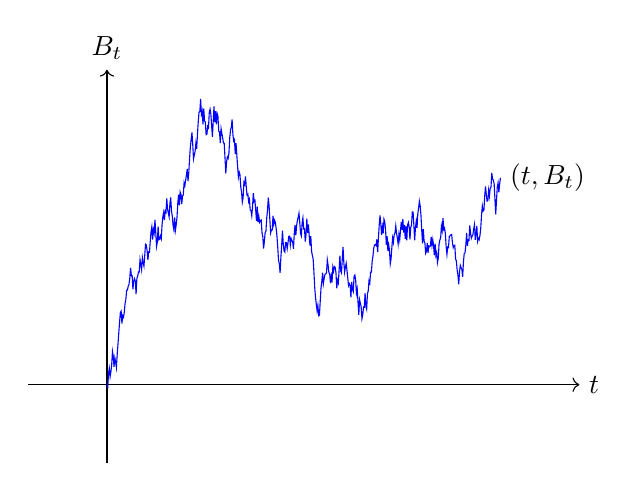
\begin{tikzpicture}
        \pgfmathsetseed{941}
      \draw[->] (-1,0) -- (6,0) node[right] {$t$};
      \draw[->] (0,-1) -- (0,4) node[above] {$B_t$};

      \draw[blue] (0,0)
      \foreach \x in {1,...,500}
      { -- ++(0.01,rand*-0.2)
      }
      node[right, black] {$(t,B_t)$};

    \end{tikzpicture}
    \caption{Primer realizacije eno-dimenzionalnega Brownovega gibanja do "casa $t$.}
    \label{fig:slika2}
\end{figure}

\section{Lastnosti}

\subsection{Osnovne lastnosti in "casi ustavljanja}

Poglejmo si nekaj osnovnih lastnosti Brownovega gibanja, ki nam bodo prišle prav v nadaljevanju 
članka.

\begin{trditev}
    Naj bo $(B_t)_{t\geq 0}$ Brownovo gibanje in $0 \leq s < t < \infty$. Potem velja:
    \begin{enumerate}
        \item $ Cov(B_t, B_s) = s$.
        \item Brownovo gibanje je simetrično, torej $(-B_{t})_{t\geq0}$ je tudi Brownovo gibanje.	
    \end{enumerate}
\end{trditev}

\begin{dokaz}
    \begin{enumerate}
        \item Ker velja $B_t - B_s \sim N(0, t-s)$, sledi
        \begin{align*}
            Cov(B_t, B_s) &= Cov(B_s + B_t - B_s, B_s) \\
                        &= Cov(B_s, B_s) + Cov(\underbrace{B_t - B_s, B_s}_{neodivsni}) \\
                        &= s + 0 = s.
        \end{align*}
        \item Zveznost realizacij, neodivsnost in stacionarnost prirastkov so lastnosti, ki se ohranjajo pri linearnih transformacijah. "Ce pogledamo razliko $(-B_t) - (-B_s)$ 
        za $0 \leq s < t$, dobimo 
        \begin{align*}
        (-B_t) - (-B_s) &= -(B_t - B_s)\\
                        &\sim -N(0, t - s)\\
                        &\sim N(0, t-s).
        \end{align*}
    \end{enumerate}
    $\hfill \square$
\end{dokaz}

%Za nadaljevanje bomo potrebovali naslednjo trditev, katere dokaz za na"se namene ni relevanten, ampak ga lahko najdemo v \cite{1}.
%
%\begin{trditev}
%    Naj bosta $X, Y$ slu"cajni spremenljivki definirani na skupnem verjetnostnem prostoru $(\Omega, \mathcal{F}, \mathbb{P})$.
%    Če velja $\mathbb{E}\left[f(X)g(X)\right] = \mathbb{E}\left[f(X)\right]\mathbb{E}\left[g(X)\right]$ za vsak par 
%     omejenih zveznih funkcij $f, g$, potem sta $X$ in $Y$ neodvisni.
%\end{trditev}

%\begin{definicija}
%    Naj bo $X$ slučajna spremenljivka defnirana na verjetnostnem prostoru $(\Omega, \mathcal{F}, \mathbb{P})$
%    in $\mathcal{G} \subseteq \mathcal{F}$ pod-$\sigma$-algebra. $X$ je \textit{neodvisna}
%    od $\mathcal{G}$, če za vsako omejeno zvezno funkcijo $f$ velja
%    $$
%        \mathbb{E}\left[f(X)\mathbbm{1}_G\right] = \mathbb{E}\left[f(X)\right]\mathbb{P}(G)
%    $$
%    za vsak $G \in \mathcal{G}$.
%\end{definicija}

\begin{definicija}
    Naj bo $(B_t)_{t\geq 0}$ Brownovo gibanje. S $\mathcal{F}_t$ 
    označimo $\sigma$-algebro generirano s $\sigma(B_s \mid 0\leq s \leq t)$. 
    Družini $(\mathcal{F}_t)_{t\geq 0}$ pravimo \textit{Brownova filtracija}.
\end{definicija}

\begin{opomba}
    V splo"snem je filtracija dru"zina nara"s"cajo"cih $\sigma$-algeber, torej $\mathcal{F}_s \subseteq \mathcal{F}_t$ za $s \leq t$, ki je lahko kon"cna ali neskon"cna.
\end{opomba}

%\begin{izrek}
%    Za vsak fiksen $t \geq 0$ je proces $\{B_{t+s}-B_t\mid s\geq 0\}$ Brownovo gibanje neodvisno 
%    od $\mathcal{F}_t$.
%\end{izrek}
%
%\begin{dokaz}
%    Naj bo $0 \leq t < \infty$ in $0 \leq s_1 < s_2 < \ldots < s_n < \infty$. 
%    Potem je $B_{t+s_1} - B_t, \ B_{t+s_2} - B_{t+s_1}, \ \ldots, \ B_{t+s_n} - B_{t+s_{n-1}}$ 
%    neodvisen od $\mathcal{F}_t$, saj je neodvisen od $B_t$ in je $\mathcal{F}_t$ generiran z 
%    $B_t$. Torej je $\{B_{t+s}-B_t\mid s\geq 0\}$ neodvisen od $\mathcal{F}_t$.
%    $\hfill \square$
%\end{dokaz}

\begin{definicija}
    Naj bo $(\mathcal{F}_t)_{t\geq0}$ filtracija. Slučajna spremenljivka $T: \Omega \rightarrow [0, \infty)\cup \{\infty\}$ 
    je \textit{čas ustavljanja} glede na filtracijo $(\mathcal{F}_t)_{t\geq0}$, če je za vsak $t \in \mathbb{R}$ dogodek $\{T \leq t\} \in \mathcal{F}_t$.
\end{definicija}

Torej če je $T$ čas ustavljanja in poznamo pot Brownovega gibanja do $t$, potem vemo, 
ali je $T\leq t$ ali ne. Poglejmo si primer časa ustavljanja in primer slučajne spremenljivke, 
ki ni čas ustavljanja.

\begin{primer}
    Naj bo $(B_t)_{t\geq0}$ Brownovo gibanje in $a \in \mathbb{R}$. Potem je
    $$
        T_a = \inf\{t \geq 0 \mid B_t = a\}
    $$
    čas ustavljanja glede na Brownovo filtracijo $(\mathcal{F}_t)_{t\geq0}$. "Se ve"c, velja $\mathbb{P}(T_a < \infty) = 1$.
\end{primer}

\begin{figure}[h]
    \centering
    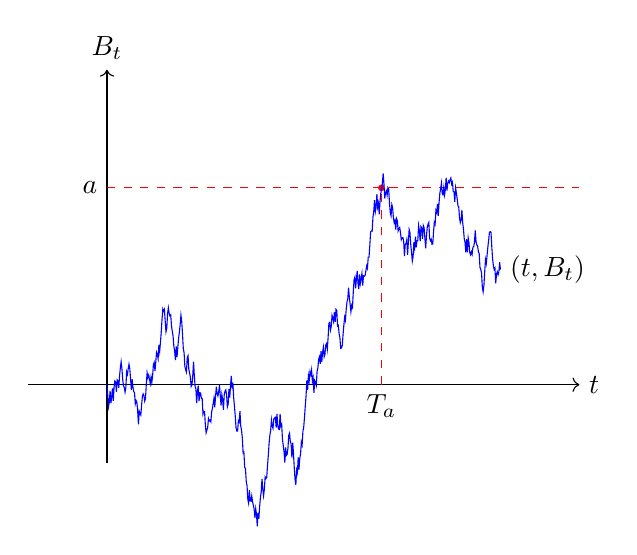
\begin{tikzpicture}
        \pgfmathsetseed{8}
        \draw[->] (-1,0) -- (6,0) node[right] {$t$};
        \draw[->] (0,-1) -- (0,4) node[above] {$B_t$};
        \draw[red, dashed] (0,2.5) -- (6,2.5);
        \draw[black] (0, 2.5) node[left] {$a$};
        \draw[red, dashed] (3.485,0) -- (3.485,2.5);
        \filldraw[red] (3.485,2.5) circle (1pt);
        \draw[black] (3.485, 0) node[below] {$T_a$};
  
        \draw[blue] (0,0)
        \foreach \x in {1,...,500}
        { -- ++(0.01,rand*-0.2)
        }
        node[right, black] {$(t,B_t)$};

    \end{tikzpicture}
    \caption{Primer realizacije $T_a$.}
    \label{fig:slika3}
\end{figure}

\pagebreak

\begin{primer}
    Naj bo $(B_t)_{t\geq0}$ Brownovo gibanje in $a < b \in \mathbb{R}$. Potem je
    $$
        T^{a, b}_{\max} = \{t \in [a, b] \mid \max\{B_t\} \}
    $$
    primer slučajne spremenljivke, ki ni čas ustavljanja glede na Brownovo filtracijo $(\mathcal{F}_t)_{t\geq0}$, saj velja npr. $\{T^{a, b}_{\max} \leq \tfrac{a+b}{2}\} \not\in \mathcal{F}_{\tfrac{a+b}{2}}$.
\end{primer}



\begin{figure}[h]
    \centering
    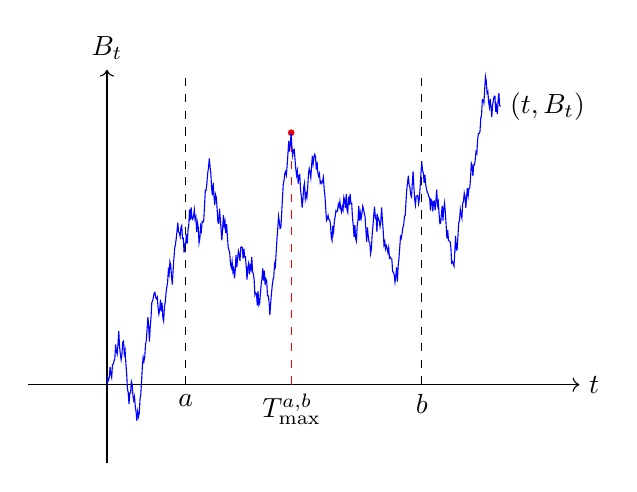
\begin{tikzpicture}
        \pgfmathsetseed{13}
        \draw[->] (-1,0) -- (6,0) node[right] {$t$};
        \draw[->] (0,-1) -- (0,4) node[above] {$B_t$};

        \draw[red, dashed] (2.34,0) -- (2.34,3.2);
        \draw[black] (2.345, 0) node[below] {$T^{a,b}_{\max}$};
        \filldraw[red] (2.34,3.2) circle (1pt);

        \draw[dashed] (1, 0) -- (1, 4);
        \draw[black] (1, 0) node[below] {$a$};

        \draw[dashed] (4, 0) -- (4, 4);
        \draw[black] (4, 0) node[below] {$b$};

        \draw[blue] (0,0)
        \foreach \x in {1,...,500}
        { -- ++(0.01,rand*-0.2)
        }
        node[right, black] {$(t,B_t)$};

    \end{tikzpicture}
    \caption{Primer realizacije $T^{a,b}_{\max}$.}
    \label{fig:slika4}
\end{figure}

Intuitivna razlaga "casa ustavljanja je naslednja. "Ce proces opazujemo do "casa $t$, potem bi radi v tem "casu imeli vse informacije, da lahko povemo
ali se je $T$ zgodil ali ne. V primeru [2] to ne velja, saj moramo vedeti vse kar se je zgodilo do "casa $b$, da lahko povemo kje je maksimum. 

\subsection{Krepka lastnost Markova}
Pokažimo, da za Brownovo gibanje velja krepka lastnost Markova. Torej, če 
v nekem trenutku ustavimo proces in ga gledamo od te točke dalje, bo neodvisen od
dotedanjega gibanja ter bo ponovno Brownovo gibanje. Prvo potrebujemo nekaj definicij in pomo"znih rezultatov, ki jih ne bomo dokazovali (dokaz lahko najdemo v \cite{1}).

%\begin{lema}
%        Naj bosta $X, Y$ slu"cajni spremenljivki definirani na skupnem verjetnostnem prostoru $(\Omega, \mathcal{F}, \mathbb{P})$.
%    Če velja $\mathbb{E}\left[f(X)g(X)\right] = \mathbb{E}\left[f(X)\right]\mathbb{E}\left[g(X)\right]$ za vsak par 
%     omejenih zveznih funkcij $f, g$, potem sta $X$ in $Y$ neodvisni.
%\end{lema}
%

\begin{definicija}
    Naj bo $X$ slučajna spremenljivka defnirana na verjetnostnem prostoru $(\Omega, \mathcal{F}, \mathbb{P})$
    in $\mathcal{G} \subseteq \mathcal{F}$ pod-$\sigma$-algebra. $X$ je \textit{neodvisna}
    od $\mathcal{G}$, če za vsako omejeno zvezno funkcijo $f$ velja
    $$
        \mathbb{E}\left[f(X)\mathbbm{1}_G\right] = \mathbb{E}\left[f(X)\right]\mathbb{P}(G)
    $$
    za vsak $G \in \mathcal{G}$.
\end{definicija}

\begin{lema}
    Naj bosta $\overline{X}, \overline{Y} $ slu"cajna vektorja. "Ce velja 
    $$
        \mathbb{E}\left[\prod_{i=1}^n f_i(X_i)\right] = \mathbb{E}\left[\prod_{i=1}^n f_i(Y_i)\right]
    $$
    za vse omejene zvezne funkcije $f_1, \ldots, f_n$ potem sta $\overline{X}$ in $\overline{Y}$ enako porazdeljena.
\end{lema}

\begin{definicija}
    Naj bo $T$ "cas ustavljanja. Potem $\sigma$-algebri
    $$
        \mathcal{F}_T = \{A \in \mathcal{F} \mid A \cap \{T \leq t\} \in \mathcal{F}_t \ za \ \forall t\}
    $$
    pravimo \textit{dogodki to "casa $T$}.
\end{definicija}

\begin{izrek}
    Naj bo $(B_t)_{t\geq 0}$ Brownovo gibanje in $T$ čas ustavljanja, za katerega velja velja $\mathbb{P}(T<\infty )=1$.
    Definiramo proces $B^*_s = B_{T + s} - B_T$ za $s\geq0$. Potem je $(B^*_s)_{s\geq0}$ Brownovo
    gibanje, neodvisno od $\mathcal{F}_T$.
\end{izrek}

\begin{dokaz}
    Predpostavino, da $T$ zavzema vrednosti v $\{0, \tfrac{1}{n}, \tfrac{2}{n}, \ \ldots, \}$ za nek $n\in\mathbb{N}$. 
    Potem za $0 \leq s_1 < s_2 < \ldots < s_n < \infty$ in $G \in \mathcal{F}_T$ ter $f_1, \ldots, f_n$ (omejene zvezne funkcije) ra"cunamo

    \begin{align*}
        \mathbb{E}\left[\prod_{k=1}^nf_k\left(B_{T+s_k} - B_{T + s_{k-1}}\right)\mathbbm{1}_G\right] &= \\
        &=\mathbb{E}\left[\prod_{k=1}^nf_k\left(B_{T+s_k} - B_{T + s_{k-1}}\right)\mathbbm{1}_G\sum_{m=0}^\infty\mathbbm{1}(T=\tfrac{m}{n})\right] \\
        &= (\text{izrek o dominirani konvergenci}) = \\
        &=\sum_{m=0}^\infty\mathbb{E}\left[\prod_{k=1}^nf_k\left(B_{T+s_k} - B_{T + s_{k-1}}\right)\mathbbm{1}_G\mathbbm{1}(T = \tfrac{m}{n})\right] = \\
        &=\sum_{m=0}^\infty\mathbb{E}\left[\prod_{k=1}^nf_k\left(B_{\tfrac{m}{n}+s_k} - B_{\tfrac{m}{n} + s_{k-1}}\right)\underbrace{\mathbbm{1}_G\mathbbm{1}(T = \tfrac{m}{n})}_{\in \mathcal{F}_{\tfrac{m}{n}}}\right] = \\
        &= \sum_{m=0}^\infty\left[\mathbb{E}\left[\prod_{k=1}^nf_k\left(B_{\tfrac{m}{n}+s_k} - B_{\tfrac{m}{n} + s_{k-1}}\right)\right]\mathbb{E}\left[\mathbbm{1}_G\mathbbm{1}(T = \tfrac{m}{n})\right]\right] = \\
        %&= ((B_{\tfrac{m}{n}+s_k}-B_{\tfrac{m}{n} + s_{k-1}})\sim (B_{s_k}-B_{s_{k-1}})) = \\
        &= \sum_{m=0}^\infty\left[\mathbb{E}\left[\prod_{k=1}^nf_k\left(B_{s_k} - B_{s_{k-1}}\right)\right]\mathbb{E}\left[\mathbbm{1}_G\mathbbm{1}(T = \tfrac{m}{n})\right]\right] = \\
        &= \mathbb{E}\left[\prod_{k=1}^nf_k\left(B_{s_k} - B_{s_{k-1}}\right)\right]\sum_{m=0}^\infty\mathbb{E}\left[\mathbbm{1}_G\mathbbm{1}(T=\tfrac{m}{n})\right] = \\
        &= \mathbb{E}\left[\prod_{k=1}^nf_k\left(B_{s_k} - B_{s_{k-1}}\right)\right]\mathbb{E}\left[\mathbbm{1}_G\sum_{m=0}^\infty\mathbbm{1}(T=\tfrac{m}{n})\right] = \\
        &= \mathbb{E}\left[\prod_{k=1}^nf_k\left(B_{s_k} - B_{s_{k-1}}\right)\right]\mathbbm{P}\left(G\right) \\
    \end{align*} 
    Pokazali smo, da ima $(B^*_s)_{s\geq0}$ naselednje lastnosti:
    \begin{enumerate}
        \item zveznost realizacij,
        \item Po lemi 3 velja, da so vektorji $(B^*_{s_2} - B^*_{s_1}, \ldots, B^*_{s_n} - B^*_{s_{n-1}})$ in $(B_{s_2} - B_{s_1}, \ldots, B_{s_n} - B_{s_{n-1}})$ enako porazdeljeni za poljuben nabor $0 \leq s_1 < s_2 < \ldots < s_n < \infty$ in prvi vektor je neodvisen od $\mathcal{F}_T$.

    \end{enumerate}
    S tem smo pokazali, da je $(B^*_s)_{s\geq0}$ Brownovo gibanje neodvisno od $\mathcal{F}_T$.
    \noindent
    Kaj pa, "ce $T$ zavzema vrednosti v $\mathbb{R}$? V tem primeru za $T$ z vrednostmi v $\{0, \tfrac{1}{n}, \tfrac{2}{n}, \ \ldots, \}$
    definiramo $T_r = \tfrac{1}{r}\lceil rT\rceil$ za $r\in\mathbb{N}$. Torej najve"cji ve"ckratnik $\tfrac{1}{r}$, ki je$ \geq T$.

    \begin{figure}[h]
        \centering
        \begin{tikzpicture}
                \draw (-1,0) -- (5,0);

                \draw (1,0) node[below] {$\frac{n-1}{r}$};
                \draw (3,0.1) -- (3,-0.1);
                \draw (3, 0) node[below] {$\frac{n}{r}$};

                \draw[->] (2.3, 0.55)--(3, 0.55);
                \draw[<-] (1,0) -- (3,0);

                \filldraw (2.3,0) circle (1pt) node[above] {$T$};

        \end{tikzpicture}
    \end{figure}
    
    \pagebreak
    \noindent
     Preverili bi lahko, da je $T_r$ res "cas ustavljanja. Ker je $T_r \geq T$ velja $\mathcal{F}_{T} \subseteq \mathcal{F}_{T_r}$. Velja $T_r \downarrow T$ ko $r \rightarrow \infty$. Torej za $G \in \mathcal{F}_T$ velja

     \begin{align*}
        &\mathbb{E}\left[\prod_{k=1}^nf_k\left(B^*_{s_k} - B^*_{s_{k-1}}\right)\mathbbm{1}_G\right] = \mathbb{E}\left[\prod_{k=1}^nf_k\left(B_{s_k} - B_{s_{k-1}}\right)\right]\mathbb{P}(G) \\
        &\mathrel{\rotatebox[origin=c]{90}{$=$}} \\
        &\mathbb{E}\left[\prod_{k=1}^nf_k\left(B_{T_r +s_k} - B_{T_r + s_{k-1}}\right)\mathbbm{1}_G\right] = \mathbb{E}\left[\prod_{k=1}^nf_k\left(B_{T_r + s_k} - B_{T_r + s_{k-1}}\right)\right]\mathbb{P}(G)
    \end{align*}

    \noindent
    Ko gre $r \rightarrow \infty$ . Po zveznosti realizacij sledi $(B_{T_r + s_k} - B_{T_r + s_{k-1}}) \rightarrow (B_{T + s_k} - B_{T + s_{k-1}})$ $\mathbb{P}$-skoraj gotovo. Zaradi dominirane konvergence lahko nesemo limito pod $\mathbb{E}$ in dobimo
    $$
        \mathbb{E}\left[\prod_{k=1}^nf_k\left(B^*_{s_k} - B^*_{s_{k-1}}\right)\mathbbm{1}_G\right] = \mathbb{E}\left[\prod_{k=1}^nf_k\left(B_{s_k} - B_{s_{k-1}}\right)\right]\mathbb{P}(G)
    $$
     $\hfill \square$
\end{dokaz}

Izrek ponazorimo s sliko \ref{fig:slika5}. "Ce Brownovo gibanje slu"cajno ustavimo in gledamo na proces od tega trenutka dalje, bo to "se vedno Brownovo gibanje. 

\begin{figure}[h]
    \centering
    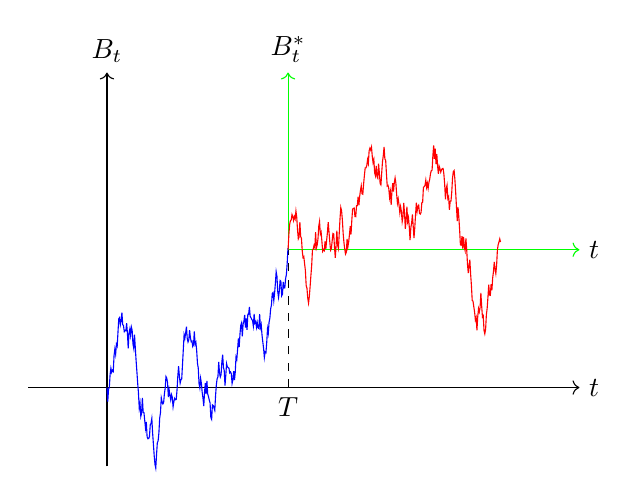
\begin{tikzpicture}
        \pgfmathsetseed{10}
        \draw[->] (-1,0) -- (6,0) node[right] {$t$};
        \draw[->] (0,-1) -- (0,4) node[above] {$B_t$};
        \draw[->, green] (2.3, 1.75) -- (6, 1.75) node[right, black] {$t$};
        \draw[->, green] (2.3, 1.75) -- (2.3, 4) node[above, black] {$B^*_t$};
        \draw[dashed] (2.3,0) -- (2.3,1.75);
        \draw[black] (2.3, 0) node[below] {$T$};
  
        \draw[blue] (0,0)
        \foreach \x in {1,...,230}
        { -- ++(0.01,rand*-0.2)
        };

        \draw[red] (2.3, 1.75)
        \foreach \x in {1,...,270}
        { -- ++(0.01,rand*-0.2)
        };

    \end{tikzpicture}
    \caption{Krepka lastnost Markova.}
    \label{fig:slika5}
\end{figure}


\subsection{Princip zrcaljenja}

Tokrat definiramo "cas ustavljanja $T_a = \inf\{t \geq 0 \mid B_t = a\}$ (glej sliko \ref{fig:slika3}, lahko bi izbrali poljuben "cas ustaljanja za katerega velj a $\mathbb{P}(T < \infty) = 1$) in v tej vrednosti glede na premico $y = a$ zrcalimo realizacijo Brownovega gibanja (glej sliko \ref{fig:slika6}). 
Krepka lastnost Markova nam pove, da je $B^*_t = B_{T_a + t} - B_{T_a}$ Brownovo gibanje neodvisno od $\mathcal{F}_{T_a}$. Vemo tudi, da je $(-B_t)_{t\geq0}$ Brownovo gibanje. Naprej od "casa $T_a$ lahko Brownovo gibanje "'podalj"samo"' s katerimkoli neodvisnim Brownovim gibanjem (neodvisnim od $\mathcal{F}_{T_a}$). Ozna"cimo to tretje Brownovo gibanje z $B'_t$. Naj bo $x<a$ realno "stevilo. Izra"cunati "zelimo 
$$
    \mathbb{P}\left(\max_{0\leq s\leq t}\{B_t\}\geq a, \ B_t \leq x\right).
$$

\begin{figure}[h]
    \centering
    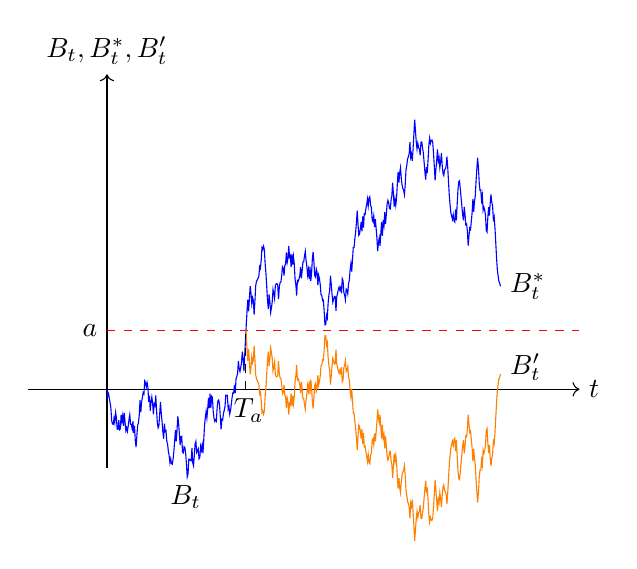
\begin{tikzpicture}
    \pgfmathsetseed{952}
    \draw[->] (-1,0) -- (6,0) node[right] {$t$};
    \draw[->] (0,-1) -- (0,4) node[above] {$B_t, B^*_t, B'_t$};
    \draw[black] (0, 0.75) node[left] {$a$};

    \draw[spath/save=horiz, red, dashed] (0,0.75) -- (6,0.75);

    \draw[blue, spath/save=squiggly] (0,0)
      foreach \x in {1,...,500}{
         -- ++(0.01,rand*-0.2) 
         }
      node[right, black] {$B^*_t$};

        \draw[
            draw=orange,
            spath/.cd,
            split at intersections with={squiggly}{horiz},
            remove components={squiggly}{1},
            use={squiggly, transform={yshift=1.5cm,yscale=-1}},
            ] node[anchor=base west] {$B'_t$};

    \draw[black, dashed] (1.76, 0) -- (1.76,0.7);
    \draw[black] (1.8, 0) node[below] {$T_a$};
    \draw[black] (1, -1.1) node[below] {$B_t$};
    \end{tikzpicture}
    \caption{Primer zrcaljenja Brownovega gibanja.}
    \label{fig:slika6}
\end{figure}

\pagebreak
\noindent
Ta verjetnost je enaka
$$
    \mathbb{P}\left(\max_{0\leq s\leq t}\{B'_t\}\geq a, \ B'_t \leq x\right),
$$
ampak ta verjetnost pa je enaka (glej sliko \ref{fig:slika6})
$$
    \mathbb{P}\left(\max_{0\leq s\leq t}\{B_t\}\geq a, \ B_t \geq 2a -x\right).
$$
"Ce velja $B_t \geq 2a - x$, velja tudi $\max_{0\leq s\leq t}\{B_t\}\geq a$. Torej je 
$$
    \mathbb{P}\left(\max_{0\leq s \leq t}\{B_t\} \geq a, \ B_t \leq x\right) = 
$$
$$
    \mathbb{P}\left(B_t \geq 2a - x\right) =
$$
$$
    1 - \varPhi\left(\frac{2a - x}{\sqrt{t}}\right),
$$
kjer je $\varPhi$ porazdelitvena funkcija normalne porazdelitve. "Ce ozna"cimo $Y_t = \max_{0\leq s\leq t}\{B_t\}$, potem je 
$$
    \mathbb{P}\left(Y_t \geq a, \ B_t \leq x\right) = 1 - \varPhi\left(\frac{2a - x}{\sqrt{t}}\right).
$$
Na"sli smo porazdelitev vektorja $(Y_t, B_t)$. Upo"stevamo, da je 
$$
    \mathbb{P}\left(Y_t \geq a, \ B_t \leq x\right) = \mathbb{P}\left(Y_t \geq a\right) - \mathbb{P}\left(Y_t \geq a, \ B_t > x\right)
$$
in ra"cunamo
\begin{align*}
    \frac{\partial^2}{\partial a \partial x}\left(1 - \varPhi\left(\frac{2a - x}{\sqrt{t}}\right)\right) &= -\frac{\partial}{\partial a}\varPhi'\left(\frac{2a - x}{\sqrt{t}}\right)\frac{1}{\sqrt{t}} =\\
    &= -\frac{\partial}{\partial a}\frac{1}{\sqrt{2\pi}}\exp\left[-\frac{(2a - x)^2}{2t}\right]\frac{1}{\sqrt{t}} =\\
    &= \frac{2(2a - x)}{\sqrt{2\pi t^3}}\exp\left[-\frac{(2a - x)^2}{2t}\right]
\end{align*}

"Ce integriramo  po $x$ do na $(-\infty, a]$ dobimo gostoto $Y_t$ 
$$
    \int_{-\infty}^a f_{Y_t, B_t}(a, x)\text{dx} = \frac{2}{\sqrt{2\pi t}}\exp\left[-\frac{a^2}{2t}\right],
$$
kar pa pomeni, da ima $Y_t$ enako porazdelitev kot $|B_t|$.

Ker za dogodek  $\{T_a \leq t\}$ velja $\{T_a \leq t\} = \{Y_t \geq a\}$ sledi 
$$
    \mathbb{P}(T_a \leq t) = \mathbb{P}(|B_t| \geq a) = 2\left(1 - \varPhi\left(\frac{a}{\sqrt{t}}\right)\right).
$$

Po odvajanju po $t$ dobimo
$$
    f_{T_a}(t) = \frac{1}{\sqrt{2\pi t^3}}\exp\left[-\frac{a^2}{2t}\right]
$$

\subsection{Neodvedljivost}
Za zaklju"cek poka"zimo "se idejo dokaza, da je realizacija Brownovega gibanja nedovedjiva povsod $\mathbb{P}$-skoraj gotovo. Potrebovali bomo naslednjo lemo.

\begin{lema}
    Naj bo $(B_t)_{t\geq 0}$ Brownovo gibanje in naj bo $a>0$ realno "stevilo. Potem je slu"cajni proces $(X_t)_{t\geq0}$ definiran s predpisom $X_t = \tfrac{1}{a}B_{a^2t}$ tudi Brownovo gibanje.
\end{lema}

\begin{dokaz}
    Zveznost realizacij, neodivsnost in stacionarnost prirastkov so lastnosti, ki se ohranjajo pri tovrstni transformaciji. "Ce pogledamo razliko $X_t - X_s$ 
    za $0 < s < t$, dobimo
    \begin{align*}
        X_t - X_s &= \tfrac{1}{a}B_{a^2t} - \tfrac{1}{a}B_{a^2s} \\
        &= \tfrac{1}{a}\left(B_{a^2t} - B_{a^2s}\right) \\
       &\sim N\left(0, \tfrac{1}{a^2}(a^2t - a^2s)\right) \\
       &\sim N(0, t-s).
    \end{align*}
    $\hfill \square$
\end{dokaz}

\begin{izrek}
    Realizacija Brownovega gibanja je nedovedljiva funkcija $\mathbb{P}$-skoraj gotovo, "se ve"c, za vsak $t > 0$ velja ali 
    $$
        \limsup_{h\to0}\tfrac{B_{t+h} - B_t}{h} = \infty \quad \text{ali} \quad \liminf_{h\to0}\tfrac{B_{t+h} - B_t}{h} = -\infty.
    $$
    ali oboje $\mathbb{P}$-skoraj gotovo.
\end{izrek}

\begin{dokaz}
    
\end{dokaz}

\begin{thebibliography}{99}

\bibitem{1} S. Roman, \emph{Introduction to mathematics of finance : from risk management to options pricing}, Science \textbf{269} (2004), 238--275. 
\bibitem{2} W. Ketterle, D.M. Kurn, D.S. Durfee, N.J. van Druten, M.R. Andrews, M.-O. Mewes in K.B. Davis, \emph{Bose-Einstein Condensation in a Gas of Sodium Atoms}, Physics Review Letters \textbf{75} (1995), 3969--3973. 


\end{thebibliography}

\end{document}
